\chapter{Introduction}
\label{sec:introduction}

This thesis revolvs around measurements involving a two photon final state.
The diphoton decay channel has been one of the two decay modes that led to the
first observation of the Higgs boson~\cite{cms_atlas_hgg_comb}. The same
final state provide a probe to test models describing new physics such as quantum gravity
effective theories based on extra dimensions or Super Symmetry (SUSY) models with an extdended
Higgs sector. The nature of the photon restrict the
particles that can decay to a two photon system to bosons with either
spin equal to zero or spin strictly greater than one~\cite{landau,yang}.
A search for beyond the standard model (BSM) resonances, performed with p-p collision data collected by the CMS experiment,
is presented in Chapter~\ref{chapter:diphotons} together with the description of the calibration procedure (Chapter~\ref{chapter:ecal}
of the detector component that contributes the most to the detection of photons in CMS (i.e. the electromagnetic calorimeter).

Measurement involving a diphton system in the final state also includes the measurement of the Higgs boson self coupling
through di-Higgs production in p-p collisions. This standard model process is extremely rare, thus its observation is
only possible with a large dataset of p-p collisions. Such dataset will be produced during the high luminosity
phase of LHC (HL-LHC), in Chapter~\ref{chapter:upgrade} the major goal and challenges of are described together with
the preliminary studies to incorporate the time information into the event reconstruction of CMS as a way to meet
the performance needed to fully exploit data collected in the high luminosity phase.

In the following sections the theoretical framework of foundamental interaction is briefly introduced.
The main focus is describe the standard model, the phenomenology of hadron collisions and the models
which gives rise to a BSM resonant diphoton production.

\section{The standard model of particle physics}
During the 20th century the development of new technologies enabled experimental
physicist to explore matter at the atomic and sub-atomic levels. At these levels
is possible to explore the building blocks of matter and the interactions between them.

A theory has been constructed during the past century which describes and predicts
a large part of the natural processes that are know today. The Standard Model of particle physics (SM)
describes in coherent way three types of interactions between sub-atomic particles:
the behavior of electromagnetic, weak and strong interaction at a quantum level is
addressed by the SM, this in fact allows us to describe a variety of phenomena with a
single mathematical framework.

The SM is build upon relativistic quantum field theory. The constituents of matter are particles
with half-integer spin that follow the Fermi-Dirac statistic while the interactions are mediated by
integer spin particles which follow Bose-Einstein statistic. Is common to refer at the first group as
fermions and to the second as bosons. Tables \ref{tab:fermions} and \ref{tab:bosons}
show the fermions and bosons described by the SM and their
main properties. 

Fermions differ from each other by mass and coupling to the force carriers, a charge is associated
to each interaction so a total of four values is used to identify a fermion: three charges and one mass.
Fermions with non-null color charge are named quarks and interact strongly with each other through the exchange
of gluons, the strong force carriers. The other fermions, called leptons, that are insensitive to
the strong force intercats interacts only electroweakly.

\begin{table}[ht]
  \begin{center}
    \begin{tabular}{|c|cc|cc|cc|c|c|}
    \hline
    & \multicolumn{2}{c|}{$1^{\textnormal{st}}$ gen.}
    & \multicolumn{2}{c|}{$2^{\textnormal{nd}}$ gen.}
      & \multicolumn{2}{c|}{$3^{\textnormal{rd}}$ gen.}
      & $Q$
      & Colour Charge \\
    \hline
    \hline
    \multirow{2}{*}{leptons} &
    \textnu$_{\textnormal{e}}$            & \small{$\sim 0$} &
    \textnu$_{\textnormal{\textmugreek}}$ & \small{$\sim 0$} &
    \textnu$_{\textnormal{\texttau}}$     & \small{$\sim 0$} &
    0 & 0 \\
    &
    e            & \small{$511 \mathrm{keV}/\mathrm{c}^2$}   &
    \textmugreek & \small{$105.7 \mathrm{MeV}/\mathrm{c}^2$} &
    \texttau     & \small{$1.777 \mathrm{GeV}/\mathrm{c}^2$} &
    -1 & 0 \\
    \hline
    \multirow{2}{*}{quarks} &
    u & \small{$1.7-3.1\mathrm{MeV}/\mathrm{c}^2$}         &
    c & \small{$1.29^{+0.05}_{-0.11}\mathrm{GeV}/\mathrm{c}^2$}  &
    t & \small{$172.9^{+1.1}_{-1.1}\mathrm{GeV}/\mathrm{c}^2$} &
    2/3 & $r,g,b$ \\
    &
    d & \small{$4.1-5.7\mathrm{MeV}/\mathrm{c}^2$} &
    s & \small{$100^{+30}_{-20}\mathrm{MeV}/\mathrm{c}^2$} &
    b & \small{$4.19^{+0.18}_{-0.06}\mathrm{GeV}/\mathrm{c}^2$} &
    -1/3 & $r,g,b$  \\
    \hline
    \end{tabular}
  \end{center}
  \linespread{1.}
  \caption{Spin-$\tfrac{1}{2}$ fermions masses and charges~\cite{PDG}.}
  \label{tab:fermions}
\end{table}

\begin{table}[ht]
  \begin{center}
    \begin{tabular}{|c|c|c|c|}
    \hline
    & Mass (GeV)
    & $Q$
    & Colour Charge \\
    \hline
      \hline
      Photon ($\gamma$) & 0 & 0 & 0 \\
      Gluon ($g$) & 0 & 0 & $r,g,b$ \\
      W & $80.385 \pm 0.015$ & $\pm 1$ & 0 \\
      Z$^0$ & $91.188 \pm 0.002$ & 0 & 0 \\
    \hline
    \end{tabular}
  \end{center}
  \linespread{1.}
  \caption{Spin-1 bosons masses and charges~\cite{PDG}.}
  \label{tab:bosons}
\end{table}

Because of the colour charges quarks can not be detected as individual particles but
only in bound states as mesons $q\bar{q}$ and barions $qqq$. This behaviour is known as
asymptotic free, i.e. he coupling is asymptotically weaker as energy increases and distance decreases
and conversely it becomes stronger at larger distances.

\section{Proton-proton collisions}
The precise measurement of the electroweak sector at the LEP and SLC electron-positron colliders and the discovery of the top
quark at Tevatron proton-antiproton collider, the yet to be oberved Higgs boson and the search for BSM physics led
to the cosntruction of the Large Hadron Collider (LHC).

Hadronic colliders, in the context of high energy physics, are great tools for discoveries since
protons are composite particles and thus both the hard scattering energy and its nature are not restricted by
the machine parameters but covers a wide range of possibilities.
The inner structure of the proton have been extensevely studied in recent years at the elctron-proton collider HERA
at DESY~\cite{hera}. The proton, as all other barions, is made of three ``valence'' quark sorrounded by a ``sea''
of gluons and quark-antiquark pairs. Quarks and gluons in this context are refered to as partons. 
This pictorical description is translated into a quantitave description by the DGLAP equations using perturbative
quatum chromodinamics (QCD)~\cite{altarelli_parisi,gribov,dokshitzer}.
The probability to find a parton carrying a fraction ``$x$'' of the total proton momentum
is described by the parton density functions (PDFs).
As shown in Figure~\ref{fig:pdfs} the valence quark dominates over the sea partons for $x>0.1$.
The PDFs depends on the momentum transfered in the scattering process, in particular for
larger values of momentum transfer $\mu^2$ the gluon PDFs dominates over the valece quark. For this reason
``gluon-fusion'' initiated provesses dominates at LHC.

\begin{figure}
  \centering
  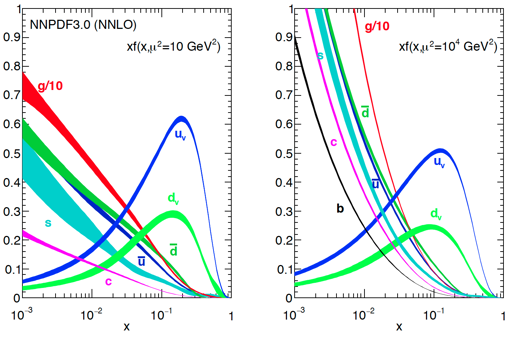
\includegraphics[width = 0.7\textwidth]{figures/introduction/pdfs.png}
  \caption{
    Distributions of $x$-times the unpolarized parton distribution function $f(x)$
    obtained in the NNPDF 3.0 global analysis at the scales of $\mu^2 = 10 \mathrm{GeV}^2$ (left) and
    $10^4 \mathrm{GeV}^2$ (right) at $\alpha_s(M_Z) = 0.118$~\cite{pdfs}.}
  \label{fig:pdfs}
\end{figure}

the perturbative QCD well describes the hard part of the hadronic collisions and the emission of
energetic quark and gluons as initial and final state radiation,
while the description of the formation of buonded QCD states from bare quark and gluons involves non-perturbative, low $\mu^2$
processes generally called ``hadronization''. 

The hadronization of quark and gluons coming from high $\mu^2$ processes (hard scattering) gives rise
to a jet of collimated hadrons , which are usually reconstructed in collider experiments as energy clusters.
The kinematic of a jet is directly linked to the one of the original quark or gluon, allowing the reconstruction
of the hard scattering.

An hard scattering usually only involves a parton from each colliding proton, the other partons interact at low $\mu^2$
(soft interactions) giving rise to the so called ``underlying event'' i.e. particles of low transverse momentum $p_T$
produced in conjuction with the bosted products of the hard interaction.

\section{Standard model diphoton production}
The main background for the search of BSM resonances decaying to two photons 